%----------------------------------------------------------------------
%----------------------------------------------------------------------
%----------------------------------------------------------------------
%	Kasutage kompileerimiseks LuaLaTeX-i.
%----------------------------------------------------------------------
%----------------------------------------------------------------------
%----------------------------------------------------------------------

\documentclass{trkut}% Reaalkooli vormistus. Muidu "report" või "article".
\usepackage[style=trkut]{biblatex}% Kasutatud kirjanduse genereerimine
\addbibresource{viited_EesnimiPerekonnanimi.bib}% Viidete info fail
\defbibheading{bibliography}{\addchap{#1}}% Lisame kasutatud materjalid sisukorda

% Siia võid lisada endale vajalikke pakke
\usepackage{listings}

\pealkiri{Gümnaasiumi uurimistöö koostamine kasutades \LaTeX \ dokumentide ettevalmistussüsteemi}
\autor{Kaarel Kivisalu}
\klass{11. a}
\juhendaja{Kaarel Kivisalu}% Juhendajad eraldada \\ sümboliga
%\toggletrue{mitujuhendajat}% Uncomment kui on mitu juhendajat (muudab sõna juhendaja(d) ja kinnituslehte)

\begin{document}
\maketitle% Tiitelleht
\tableofcontents% Sisukord

\addchap{Sissejuhatus}
\nummerdame% See käsk peab olema õigeks nummerdamiseks kohe peale sissejuhatust

Uurimistöös käsitletakse \LaTeX \ dokumentide ettevalmistussüsteemi kasutamist gümnaasiumi uurimistöö koostamiseks. Autor on koostanud Tallinna Reaalkooli nõuetele vastava alusfaili dokumentide vormistamiseks. 

Kui kirjutada urimistööd matemaatilistel või tehnilistel teemadel (ei pea tingimata olema nendel teemadel), siis luues see kasutades \LaTeX'i on soovitatav, kuna võimaldab keskenduda töö kirjutamisele vormistusle mõtlemata. \LaTeX \ on võimeline profesionaalselt vormindama dokumente, mis on sadu või tuhandeid lehekülgi pikad. Lihtsate märgenduskäskudega loob \LaTeX \ automaatselt sisukorra, äärised, päised, jalused ja hoiab vorminduse järjepidava ja kauni. Üks suuremaid tugevusi on võimekus kergesti vormindada isegi keerulist matemaatikat.

\LaTeX \ ei ole \textsc{WYSIWYG} (ingl \textit{What You See is What You Get}) programm nagu Microsoft Word või Google Docs. \LaTeX'is koostatud failid on lihtsad tekstifailid ja neis puudub vormindus. See saadaks lõppdokumenti lihtsate käskudega, mis on teksti sees. See tähendab, et \LaTeX \ on märgistuskeel nagu HTML.

\chapter{\LaTeX \ sisendfail}
\LaTeX'i sisendfailiks on tekstifail. Väljundfaili saamiseks on vaja kompileerida. Tallinna Reaalkooli uurimistööde alusfaili kasutades on vaja selleks kasutada LuaLaTeX'i. Uurimistöö autor soovitab kasutada töö kirjutamiseks pilves Overleaf'i või Windowsis MiKTeX'i ja TeXStudio't. Sobivad programmid on olemas ka Linux'is.

Ühele reale on mõistlik kirjutada kas lõik või lause. Uue lõigu alustamiseks tuleb jätta tühi rida. Mitu järjestikust tühikut loetakse üheks.

Kasulikuks kohaks õppimisel on \url{https://www.overleaf.com/learn/latex/Main_Page}.

\section{Erimärgid}
Osad märgid on reserveeritud vormindamise jaoks. Nende kirjutamiseks on vaja enne neid sisestada \textbackslash. Märkide \# \$ \% \^{} \& \_ \{ \} \~{} \textbackslash saab kasutada järgmisi käske:
\begin{verbatim}
    \# \$ \% \^{} \& \_ \{ \} \~{} \textbackslash 
\end{verbatim}

\verb!\\! käsk on reserveeriud uue rea jaoks. Selle kasutamist võiks vältida, kuna võib rikkuda vormistust.

\section{Joonised}\label{sec:1}
Jooniseid saab lisada kasutades \verb!figure! keskkonda. Joonis \ref{joonis1} on lisatud kasutades järgnevaid käske:
\begin{verbatim}
\begin{figure}[htb]% [] sisse märgitakse paigutus !htbp
	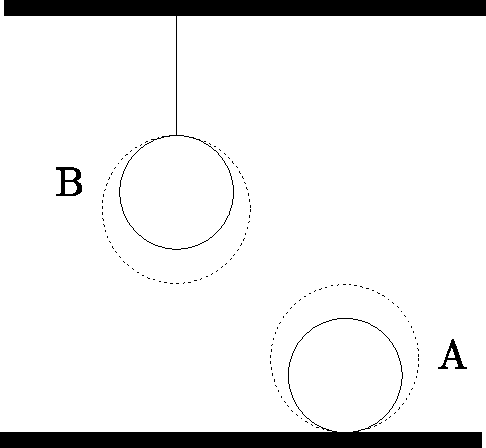
\includegraphics[5cm]{joonis1.pdf}% Joonise suurus, joonise fail
	\caption{Probleemi ülesehitus}% Allkiri
	\allikas{Autori andmed}% Allikas
	\label{joonis1}% Selle järgi viidatakse, pärast käsku \caption
\end{figure}
\end{verbatim}
\begin{figure}[htb]% [] sisse märgitakse paigutus !htbp
	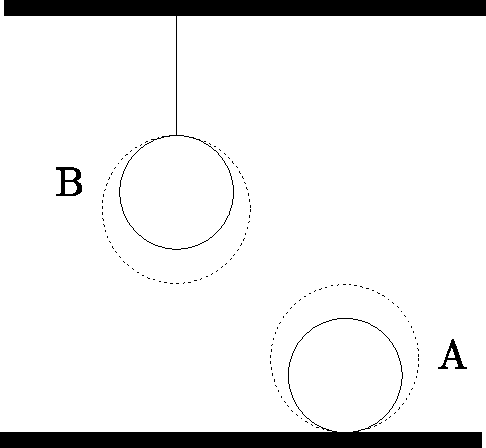
\includegraphics[width=5cm]{joonis1.pdf}% Joonise suurus, joonise fail
	\caption{Probleemi ülesehitus}% Allkiri
	\allikas{Autori andmed}% Allikas
	\label{joonis1}% Selle järgi viidatakse, pärast käsku \caption
\end{figure}

\section{Tabelid}
Tabeleid saab koostada kasutades \verb!table! ja \verb!tabular!. Kuna pikkade tabelite vormistamine \LaTeX'is on tülikas, siis on võimalik ka lisada tabel \verb!csv! failist. Tabel \ref{tabel1} on lisatud kasutades järgnevaid käske:
\begin{verbatim}
\begin{table}[htb]
	\caption{Eksperimentaalsed andmed}% Pealkiri
	\label{tabel1}% Tabelile viitamine
	\begin{tabular}{r|r|r}% r - paremjoondatud tulp, | - püstjoon
		\hline% Horisontaalne joon
		Tulp 1 & Tulp 2 & Tulp 3 \\% Märgiga & eraldatakse tulbad
		\hline
		... & ... & ... \\
		... & ... & ... \\
		... & ... & ... \\
		... & ... & ...
	\end{tabular}
	\allikas{Autori andmed}}% Viide
\end{table}     
\end{verbatim}

\begin{table}[htb]
	\caption{Tabeli pealkiri}% Pealkiri
	\label{tabel1}% Tabelile viitamine
	\begin{tabular}{r|r|r}% r - paremjoondatud tulp, | - püstjoon, lrcp on võimalikud käsud
		\hline% Horisontaalne joon
		Tulp 1 & Tulp 2 & Tulp 3 \\% Märgiga & eraldatakse tulbad
		\hline
		... & ... & ... \\
		... & ... & ... \\
		... & ... & ... \\
		... & ... & ...
	\end{tabular}
	\allikas{Autori andmed}% Viide
\end{table} 

\section{Valemid}
Teksisiseste valemite vormistamiseks saab kasutada käsku \verb!\( \)! või \verb!$ $!. Näiteks valemi \( a^2+b^2=c^2\) saamiseks on kasutatud käsku \verb!\( a^2+b^2=c^2\)!.

Eraldi real olevate tabelite vormistamiseks on kaks võimalust. Ilma nummerdamata vormistamisks saab kasutada käsku \verb!\[ \]! või \verb!$$ $$!. Näiteks valemi 
\[\int_{-\infty}^{+\infty} e^{-x^2} dx = \left( 6 \sum_{n=1}^{\infty} \frac{1}{n^2} \right)^\frac{1}{4}\]
saamiseks on kasutatud käsku 
\begin{verbatim}
    \[\int_{-\infty}^{+\infty} e^{-x^2} dx =
    \left( 6 \sum_{n=1}^{\infty} \frac{1}{n^2} \right)^\frac{1}{4}\]
\end{verbatim}

Nummerdusega valemite saamiseks on vaja kasutada keskkonda \verb!equation!. Valemi \ref{eq1} on lisatud kasutades järgnevaid käske: 
\begin{verbatim}
\begin{equation}\label{eq1}
    \int_{-\infty}^{+\infty} e^{-x^2} dx =
    \left( 6 \sum_{n=1}^{\infty} \frac{1}{n^2} \right)^\frac{1}{4}.
\end{equation}    
\end{verbatim}

\begin{equation}\label{eq1}
    \int_{-\infty}^{+\infty} e^{-x^2} dx = \left( 6 \sum_{n=1}^{\infty} \frac{1}{n^2} \right)^\frac{1}{4}.
\end{equation} 

\section{Failid}
Lisaks põhifailile on kompileerimiseks vajalikud ka muud failid. Kompileerimise käigus loovad \LaTeX\ ja BibLaTeX ka muid faile, nende pärast pole vaja muretseda.

\verb!135d_EesnimiPerekonnanimi.tex! -- see  on fail, mille järgi \LaTeX\ kompileerib uurimistöö \verb!.pdf! failiks. Siia on kirjutatud kogu uurimistöö (või on siin lisatud osad, mis on eraldi failidena kirjutatud).

\verb!trkut.cls! -- see  on class fail, mille järgi \LaTeX\ vormistab uurimistöö.

\verb!135d_EesnimiPerekonnanimi.pdf! -- see on  \LaTeX'i  vormistatud uurimistöö \verb!.pdf! formaadis.

\verb!viited_EesnimiPerekonnanimi.bib! -- see on oluline fail, kus on kõik informatsioon kasutatud materjalidele, millele tahad viidata. Selle faili võib ise kirjutada, kuid parem on lasta see automaatselt koostada, milleks on võimelised paljud kasutatud materjalide haldajad.

\verb!trkut.cbx! -- see on oluline fail, kus on kirjas Tallinna Reaalkooli viidete vormistamise stiil.

\verb!trkut.bbx! -- see on oluline fail, kus on kirjas Tallinna Reaalkooli kasutatud materjali vormistamise stiil.

\verb!estonian.lbx! -- see on eesti keele toetamisks vajalik fail. Ei ole alati vajalik.

\verb!135d_EesnimiPerekonnanimi.aux! -- see on \LaTeX'i genereeritud abifail, kui see kustutatakse, siis \LaTeX genereerib selle uuesti \verb!135d_EesnimiPerekonnanimi.tex! kompileerimisel. 

\verb!135d_EesnimiPerekonnanimi.bbl! -- see on BibLaTex'i genereeritud lisafail, kui see kustutatakse, siis BibLaTeX genereerib selle vajadusel uuesti. Siin on materjalid, millele on tegelikult töös viidatud. Selle järgi koostatakse kasutatud materjalid.

\verb!135d_EesnimiPerekonnanimi.blg! -- BiBLaTeX'i genereeritud lisafail. 

\verb!135d_EesnimiPerekonnanimi.lof! -- \LaTeX'i genereeritud lisafail. Selle järgi luuakse jooniste sisukord.

\verb!135d_EesnimiPerekonnanimi.log! -- \LaTeX'i genereeritud lisafail. Siin asuvad veateated.

\verb!135d_EesnimiPerekonnanimi.lot! -- \LaTeX'i genereeritud lisafail. Selle järgi luuakse tabelite sisukord.

\verb!135d_EesnimiPerekonnanimi.out! -- \LaTeX'i genereeritud lisafail.

\section{Peatükid}
Pealkirjade ja alapealkijade jaoks on olemas järgmised käsud: 
\begin{verbatim}
\chapter{Pealkiri 1}
\section{Pealkiri 1.1}
\subsection{Pealkiri 1.1.1}
\subsubsection{Pealkiri 1.1.1.1}
\paragraph{Pealkiri 1.1.1.1.1}
\subparagraph{Pealkiri 1.1.1.1.1.1}
\end{verbatim}

Ilma nummerduseta pealkirjaks on vaja kasutada käsku \verb!\addchap{}!. Käsk \verb!\chapter*{}! ei lisa pealkirja sisukorda. 

\subsection{Lisad}
Lisasid saab koostada peale käsku \verb!\appendix!. Lisade pealkirjade nummerdus on automaatne. Tuleb vaid lisada pealkiri käsuga \verb!\chapter{}!.

\section{Pakid}
Alusfail toetab mitmeid autorile kasulikke pakke. Nende loetelu ja kirjelus on toodud allpool. Kui soovitud pakki pole loetelus, siis saab selle lisada käsuga \verb!\usepackage{}!.
\subsection{\textsf{csquotes}}
Selle pakiga saab kasutada eesti jutumärke käsuga \verb!\enquote{}!.
\subsection{\textsf{graphicx}}
Selle pakiga saab lisada jooniseid. Vaata peatükki \ref{sec:1} lisainfo jaoks.
\subsection{\textsf{amsmath} ja \textsf{amssymb}}
Suurendavad matemaatiliste tehete võimalusi.
\subsection{\textsf{hyperref}}
See pakk koostab \file{.pdf} failide metadata. Käsuga \url{} saab koostada hüperlinke.
\subsection{\textsf{siunitx}}
SI ühikute ja arvude vormistamiseks on see soovitatav. Tagab ühtse stiili igal pool. Saab kasutada valemite sees. Näide:
\begin{verbatim}
\num{125,5e2}\\
\si{\kg\squared\per\Pa\tothe{4}}\\
\SI{125,5e2}{\kg\squared\per\Pa\tothe{4}}
\end{verbatim}
\num{125,5e2}\\
\SI{5}{\degree}\\
\si{\kg\squared\per\Pa\tothe{4}}\\
\SI{125,5e2}{\kg\squared\per\Pa\tothe{4}}


\chapter{Kasutatud materjalid ja viitamine BibLaTeX'iga}
Alusfail töötab \verb!biblatex! pakiga. See koostab automaatselt viited ja kasutatud materjalide loetelu. Kõik materjalid, millele viidatakse peavad olema kirjas \verb!.bib! failis. 

\section{Viited}
Tekstisiseseid viiteis saab luua käsuga \verb!\cite{}!. Praegu pole see korrektselt vormistatud, aga selle pärast pole vaja praegu muretseda. \cite{palma15}

\section{Kasutatud materjalid}
Kasutatud materjalide loetelu koostatakse viidete alusel käsuga \verb!\printbibliography!. Kui on soov testida kasutatud materjale isegi kui neile pole viidatud, siis võib kasutada käsku \verb!\nocite{*}! kõikide materjalide või \verb!\nocite{}! üksiku materjali jaoks. \cite{palma15}[1-5]

\addchap{Kokkuvõte}

\nocite{*}
\printbibliography

\appendix

\chapter{Kogu selle faili kood}
\tiny
\lstinputlisting[breaklines]{135d_EesnimiPerekonnanimi.tex}
\normalsize

\kinnitusleht
\end{document}
